\section{Implementierung}

In diesem Kapitel wird die Implementierung des Projektes mit Fokussierung auf die einzelnen Komponenten beschrieben.

\subsection{Kommunikation}

Die Kommunikation zwischen den einzelnen Komponenten des Schwarmverhaltens baut auf einer klaren Struktur für eine klare Definition zur gegenseitigen Interpretation auf, siehe \ref{fig:full_classdiagram}. Dabei stehen die dargestellten Command Objekte im Vordergrund, die die einzelnen Datenobjekte darstellen, die zur Kommunikation verwendet werden. Die restlichen stellen die Datenobjekte, mit der Identifizierung sowie den erfassten Daten von App und Robot, die zur STeuerung beitragen.

\begin{figure}[h]
	\begin{center}
		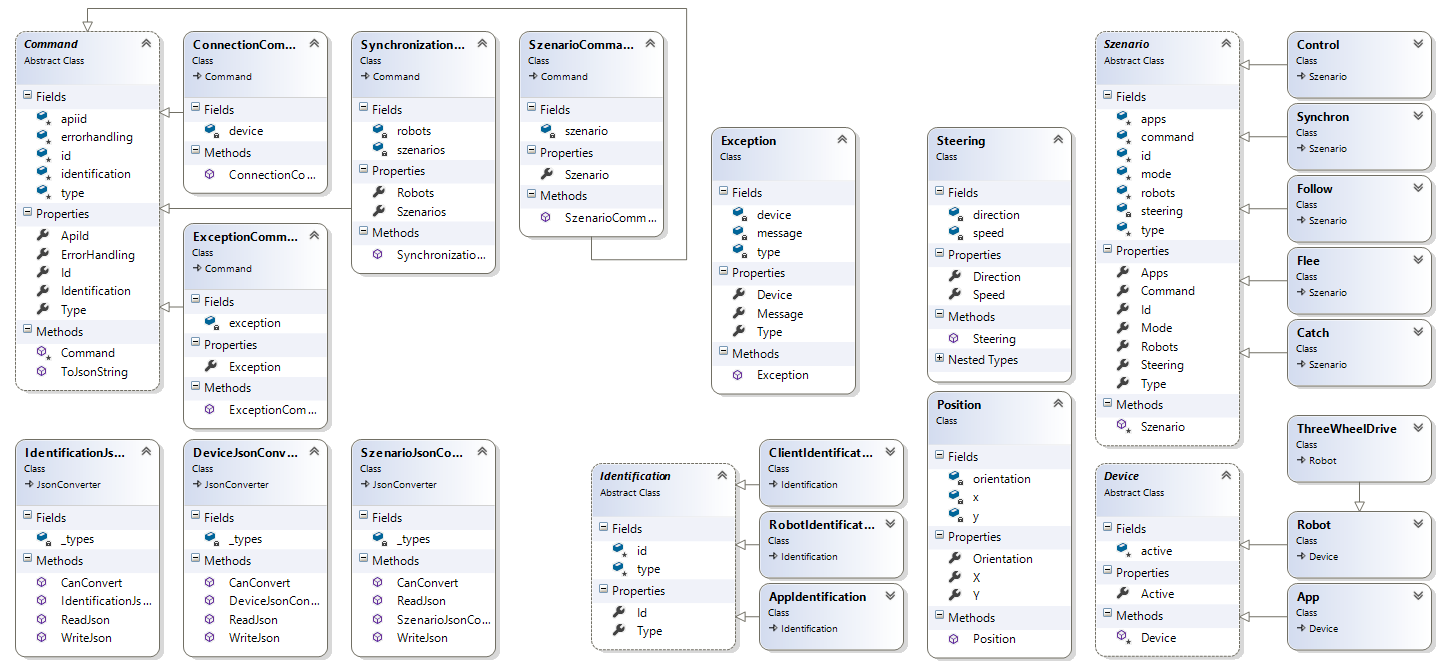
\includegraphics[width=0.95\textwidth]{images/uml/full_class_diagram.png}
	\end{center}
	\caption{Aufbau Commands}
	\label{fig:full_classdiagram}
\end{figure}

\newpage
Die Command Objekte stellen die Basis der Kommunikationstruktur und sind nach einer definierten STruktur aufgebaut, siehe ??. Diese entalten dabei die allgemeinen Identifikations Objekte, sowie die Daten, die der Steuerung des Schwarmverhaltens zugrunde liegen.

\begin{figure}[h]
	\begin{center}
		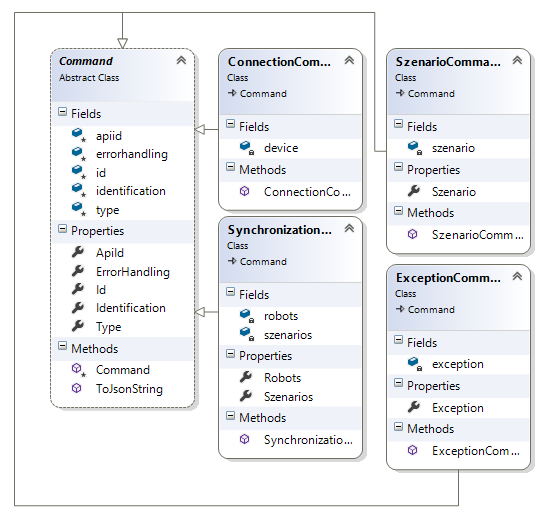
\includegraphics[width=0.6\textwidth]{images/uml/commands.png}
	\end{center}
	\caption{Commands}
	\label{fig:commands_classdiagram}
\end{figure}

\newpage
Die Identifikations Objekte stellen wie ihr Name die einzlnen Komponenten, mit ihren definierten Attributen dar un dienen eldiglich der Identifikation, von welcher Komponente das aktuelle KOmmando stammt. DIese Objekte sind daher in allesn definierten Kommandos zu finden.

\begin{figure}[h]
	\begin{center}
		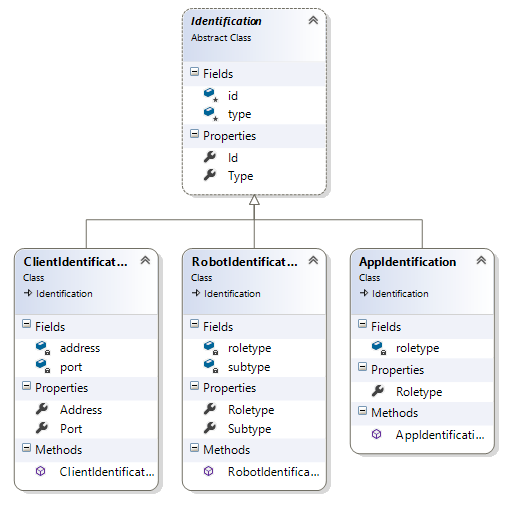
\includegraphics[width=0.6\textwidth]{images/uml/identification.png}
	\end{center}
	\caption{Identifications}
	\label{fig:identification_classdiagram}
\end{figure}

\newpage
Die Device Objekte stellen die KOmponenten im ganzen dar und enthalten zu speziellen Identifikations Attribute die allgemeinen Daten, sowie die Steuerungsoperatoren. Dabei wird unter den zwei existierenden KOmponenten unterschieden und kann durch einen vorliegenden COnverter serialisiert werden.

\begin{figure}[h]
	\begin{center}
		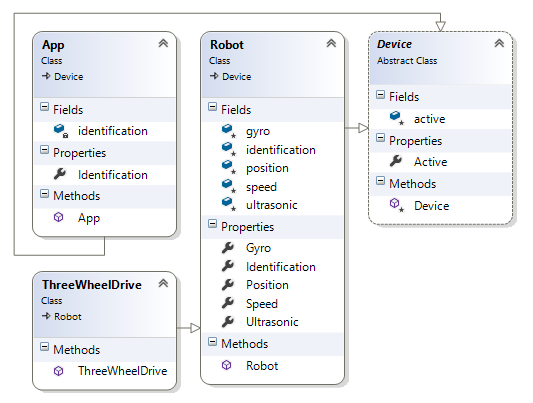
\includegraphics[width=0.6\textwidth]{images/uml/devices.png}
	\end{center}
	\caption{Devices}
	\label{fig:devices_classdiagram}
\end{figure}

\newpage
Die Szenarios stellen den aktuellen Kontext des Schwarmverhaltens dar und enthalten zu Identifikations Attributen zusätzliche die teilnehmenden Devices um diese zuordnen zu könnn. Diese Objekte werden laufend aktualisiert und haben nur zur Laufzeit des entsprechenden Szenarios ihre Gültigkeit, wobei sie bei Beendigung gelöscht werden.

\begin{figure}[h]
	\begin{center}
		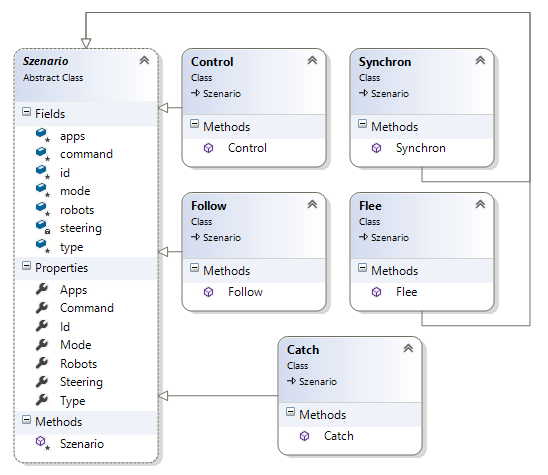
\includegraphics[width=0.6\textwidth]{images/uml/szenarios.png}
	\end{center}
	\caption{Scenarios}
	\label{fig:szenarios_classdiagram}
\end{figure}

\newpage
Um Objekte spezifisch zu abstrahieren, werden sogenannte Converter verwendet, um abstrahierte Objekte direkt abgeleiteten Klassen zuzuordenn und entsprechende Programmlogik auszuführen. Dabei wird auf die entsprechende Bibliothek mit Grundlogik zurückgegriffen und entsprechende Bedingungen hinzugefügt. siehe \ref{fig:converter_classdiagram}

\begin{figure}[h]
	\begin{center}
		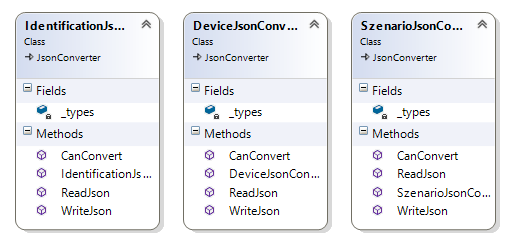
\includegraphics[width=0.6\textwidth]{images/uml/json_converter.png}
	\end{center}
	\caption{JSON Converter}
	\label{fig:converter_classdiagram}
\end{figure}

\newpage
\subsection{App}

\subsubsection{Workflow} %Struktur

\paragraph{Design Pattern}
\paragraph{\acrfull{mvvm}}
\paragraph{Bindings}

\subsubsection{\acrfull{gui}} %Oberfläche

\subsubsection{Buisnesslogic} %Logik

\subsection{Backend}

\begin{comment}
Aufbau
Interpreter
Mechanismen
GUI
\end{comment}

\subsection{Robot}

\begin{comment}
Aufbau
Robot
RobotController
EV3 Library
GUI
\end{comment}